\documentclass[border=10pt]{standalone}
\usepackage{tikz}
\usetikzlibrary{calc,positioning,shapes.geometric}

\begin{document}

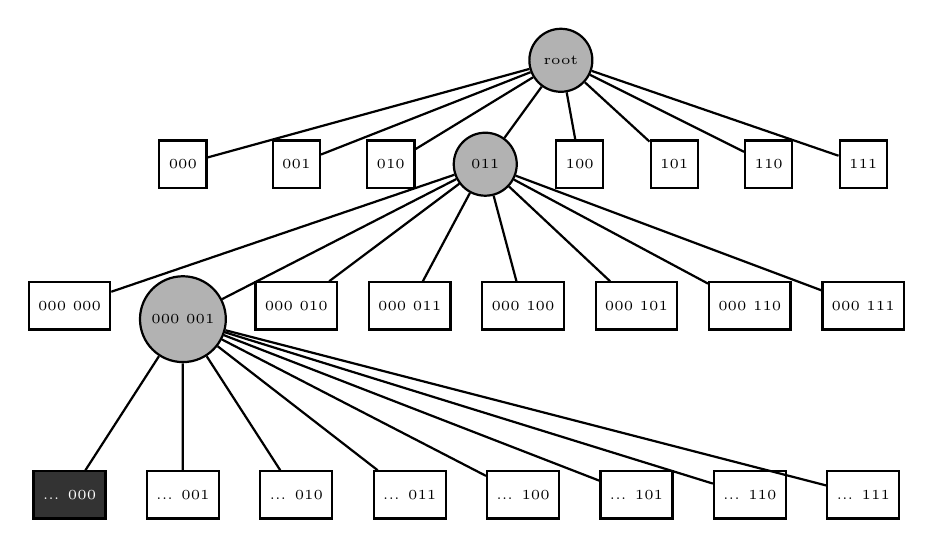
\begin{tikzpicture}[
    scale=1.2,
    node/.style={circle, draw, thick, minimum size=0.8cm},
    leaf/.style={rectangle, draw, thick, minimum size=0.6cm},
    morton/.style={font=\tiny, color=blue!70!black},
    level/.style={font=\scriptsize, color=red!70!black}
]

% Right side: Tree representation
\begin{scope}[xshift=4cm]
    % Root node (Level 0)
    \node[node, fill=gray!60] (root) at (0,-0.4) {\tiny root};
    
    % Level 1 children
    \node[leaf, fill=white] (n1) at (-4,-1.5) {\tiny 000};
    \node[leaf, fill=white] (n2) at (-2.8,-1.5) {\tiny 001};
    \node[leaf, fill=white] (n3) at (-1.8,-1.5) {\tiny 010};
    \node[node, fill=gray!60] (n4) at (-0.8,-1.5) {\tiny 011};
    \node[leaf, fill=white] (n5) at (0.2,-1.5) {\tiny 100};
    \node[leaf, fill=white] (n6) at (1.2,-1.5) {\tiny 101};
    \node[leaf, fill=white] (n7) at (2.2,-1.5) {\tiny 110};
    \node[leaf, fill=white] (n8) at (3.2,-1.5) {\tiny 111};

    % Level 2 children (only for node 1)
    \node[leaf, fill=white] (n10) at (-5.2,-3) {\tiny 000 000};
    \node[node, fill=gray!60] (n11) at (-4,-3.14) {\tiny 000 001};
    \node[leaf, fill=white] (n12) at (-2.8,-3) {\tiny 000 010};
    \node[leaf, fill=white] (n13) at (-1.6,-3) {\tiny 000 011};
    \node[leaf, fill=white] (n14) at (-0.4,-3) {\tiny 000 100};
    \node[leaf, fill=white] (n15) at (0.8,-3) {\tiny 000 101};
    \node[leaf, fill=white] (n16) at (2,-3) {\tiny 000 110};
    \node[leaf, fill=white] (n17) at (3.2,-3) {\tiny 000 111};

    % Level 3 children (only for node 1)
    \node[leaf, fill=black!80, text=white] (n18) at (-5.2,-5) {\tiny ... 000};
    \node[leaf, fill=white] (n19) at (-4,-5) {\tiny ... 001};
    \node[leaf, fill=white] (n20) at (-2.8,-5) {\tiny ... 010};
    \node[leaf, fill=white] (n21) at (-1.6,-5) {\tiny ... 011};
    \node[leaf, fill=white] (n22) at (-0.4,-5) {\tiny ... 100};
    \node[leaf, fill=white] (n23) at (0.8,-5) {\tiny ... 101};
    \node[leaf, fill=white] (n24) at (2,-5) {\tiny ... 110};
    \node[leaf, fill=white] (n25) at (3.2,-5) {\tiny ... 111};

    % Edges from root to level 1
    \draw[thick] (root) -- (n1);
    \draw[thick] (root) -- (n2);
    \draw[thick] (root) -- (n3);
    \draw[thick] (root) -- (n4);
    \draw[thick] (root) -- (n5);
    \draw[thick] (root) -- (n6);
    \draw[thick] (root) -- (n7);
    \draw[thick] (root) -- (n8);
    
    % Edges from node 1 to level 2
    \draw[thick] (n4) -- (n10);
    \draw[thick] (n4) -- (n11);
    \draw[thick] (n4) -- (n12);
    \draw[thick] (n4) -- (n13);
    \draw[thick] (n4) -- (n14);
    \draw[thick] (n4) -- (n15);
    \draw[thick] (n4) -- (n16);
    \draw[thick] (n4) -- (n17);

    % Edges from node 2 to level 3
    \draw[thick] (n11) -- (n18);
    \draw[thick] (n11) -- (n19);
    \draw[thick] (n11) -- (n20);
    \draw[thick] (n11) -- (n21);
    \draw[thick] (n11) -- (n22);
    \draw[thick] (n11) -- (n23);
    \draw[thick] (n11) -- (n24);
    \draw[thick] (n11) -- (n25);
\end{scope}

\end{tikzpicture}

\end{document}